\documentclass[a4paper,11pt]{article}
\usepackage[utf8]{inputenc}
\usepackage{graphicx}
\usepackage[a4paper]{geometry} %pour les marges
\geometry{hscale=0.77,vscale=0.85,centering}

\title{Configuration de routeur Cisco}
\author{Groupe 1\\Alicia \textsc{Galina}, Corentin \textsc{Ducruet}, Jason \textsc{Bury}, Ishène \textsc{Porteur}}
\date{5 octobre 2016}
\begin{document}
\maketitle

\section{Introduction}
En suivant une certaine topologie (figure \ref{fig:topo}),
nous devions d'abord configurer le routeur qui nous était attribué pour que nous puissions envoyer des pings aux PC des autres membres de notre groupe,
c'est à dire aux PC faisant partie de notre VLAN.
Ensuite, il fallait configurer notre routeur pour pouvoir envoyer des pings aux PC faisant partie d'autres VLAN.
Notre groupe est le groupe 1.
\begin{figure}
 \centering
 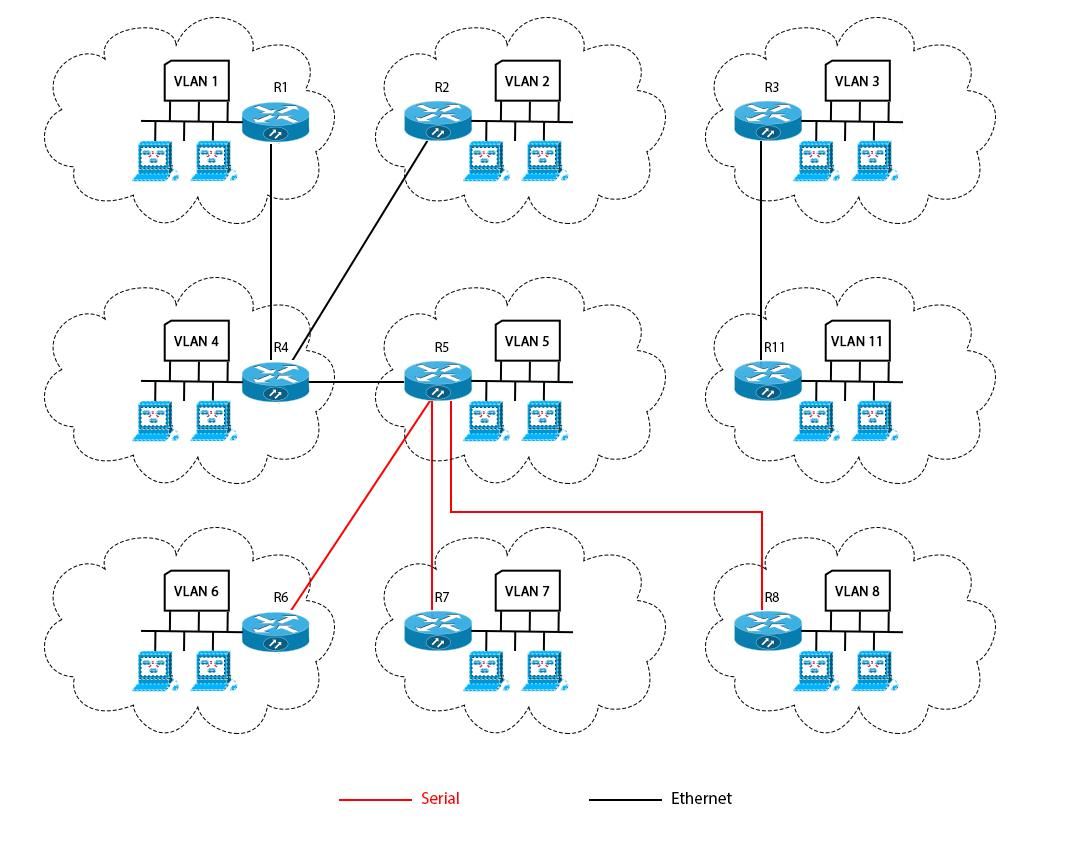
\includegraphics[height=7cm]{topo.jpg}
 \caption{Topologie à suivre pour ce travail pratique}
 \label{fig:topo}
\end{figure}

\section{Configuration}
\subsection{Se connecter}
Une fois connecté au \textit{Secure Console Server} du routeur R1 via l'Access Point sans-fil, Nous accèdons à l'invite de commande du routeur.
La commande suivante nous permet de passer en mode privilégié.
\begin{verbatim}
R1>enable
\end{verbatim}
Notre routeur a deux interfaces:
\begin{itemize}
 \item \textbf{Interface 1/0:} Faisant partie du sous-réseaux contenant notre VLAN.
 \item \textbf{Interface 0/0:} Faisant partie du sous-réseaux contenant R1 et R4 et la connection Point-to-point entre eux.
\end{itemize}
L'étape suivante consiste donc à configurer l'interface 1/0.
Les IP des réseaux attribués aux groupes sont de la forme 192.168.10$X$.0 où $x$ est le numéro de groupe.
Nous avons choisis d'attribuer à cet interface la plage d'IP correspondant à 192.168.101.1 avec le masque 255.255.255.240.
%TODO Ishene , justification du masque
\begin{verbatim}
R1#conf t
R1(config)#int Ethernet1/0
R1(config-if)#ip address 192.168.101.1 255.255.255.240
R1(config-if)#no shutdown
R1(config-if)#exit
\end{verbatim}
Depuis un PC connecté manuellement à notre VLAN, un ping a été envoyé au routeur avec succès.

\end{document}